\chapter{Search Strategy} \label{chapter-method}

\section{Strategy Overview}
A data-driven method is used to predict the background yield in the
signal regions, as well as the uncertainties on those
predictions. First, jet mass templates are created from control region jets.
Randomized jet masses, known as dressed masses, are generated from
these templates for each jet in the kinematic sample. Summing the
dressed masses for each of the up to four leading jets in an event gives the
dressed $M_{J}^{\Sigma}$ for that event. The dressed $M_{J}^{\Sigma}$
distribution for each signal region is
used to estimate the expected background contribution to that region.

\section{Discriminating Variables}
Two of the main discriminating observables, namely $M_J^{\Sigma}$ and
$|\Delta\eta_{12}|$ are the same as those used in the Run-1 version of
the analysis \cite{run1-multijet}. 

The first observable,
$M_J^{\Sigma}$, is the scalar sum of the first four leading large-R jets,
ordered by $p_{T}$, in an event. Large-R jets have $R=1.0$ and are
required to have $p_{T} > 200~GeV$ and $|\eta|<2.0$. In case an event has less than four
jets, the sum of all large-R jet masses passing the kinematic cuts is
used.

$M_{J}^{\Sigma}$ provides good separation between signal and
background because it takes into
account both the energy and angular structure of an event, unlike a
purely energy-dependent observable like $H_{T}$ \cite{hook-mj,
  elhedri-mj}.

The second discriminating variable is $|\Delta \eta_{12}|$, which is
the pseudorapidity differences between the first two leading jets in
an event. Events with small $|\Delta \eta_{12}|$ have their leading
two jets more central than average. For regions with high jet
multiplicity, requiring large $|\Delta \eta_{12}|$ reduces the signal
to background ratio, allowing for the creation of high-multiplicity
control and signal regions.

Distributions of the two discriminating variables are shown in figure
\ref{fig:MJ_dEta_distributions_combined} for data as well as
background and signal Monte Carlo.

\begin{figure}[h]
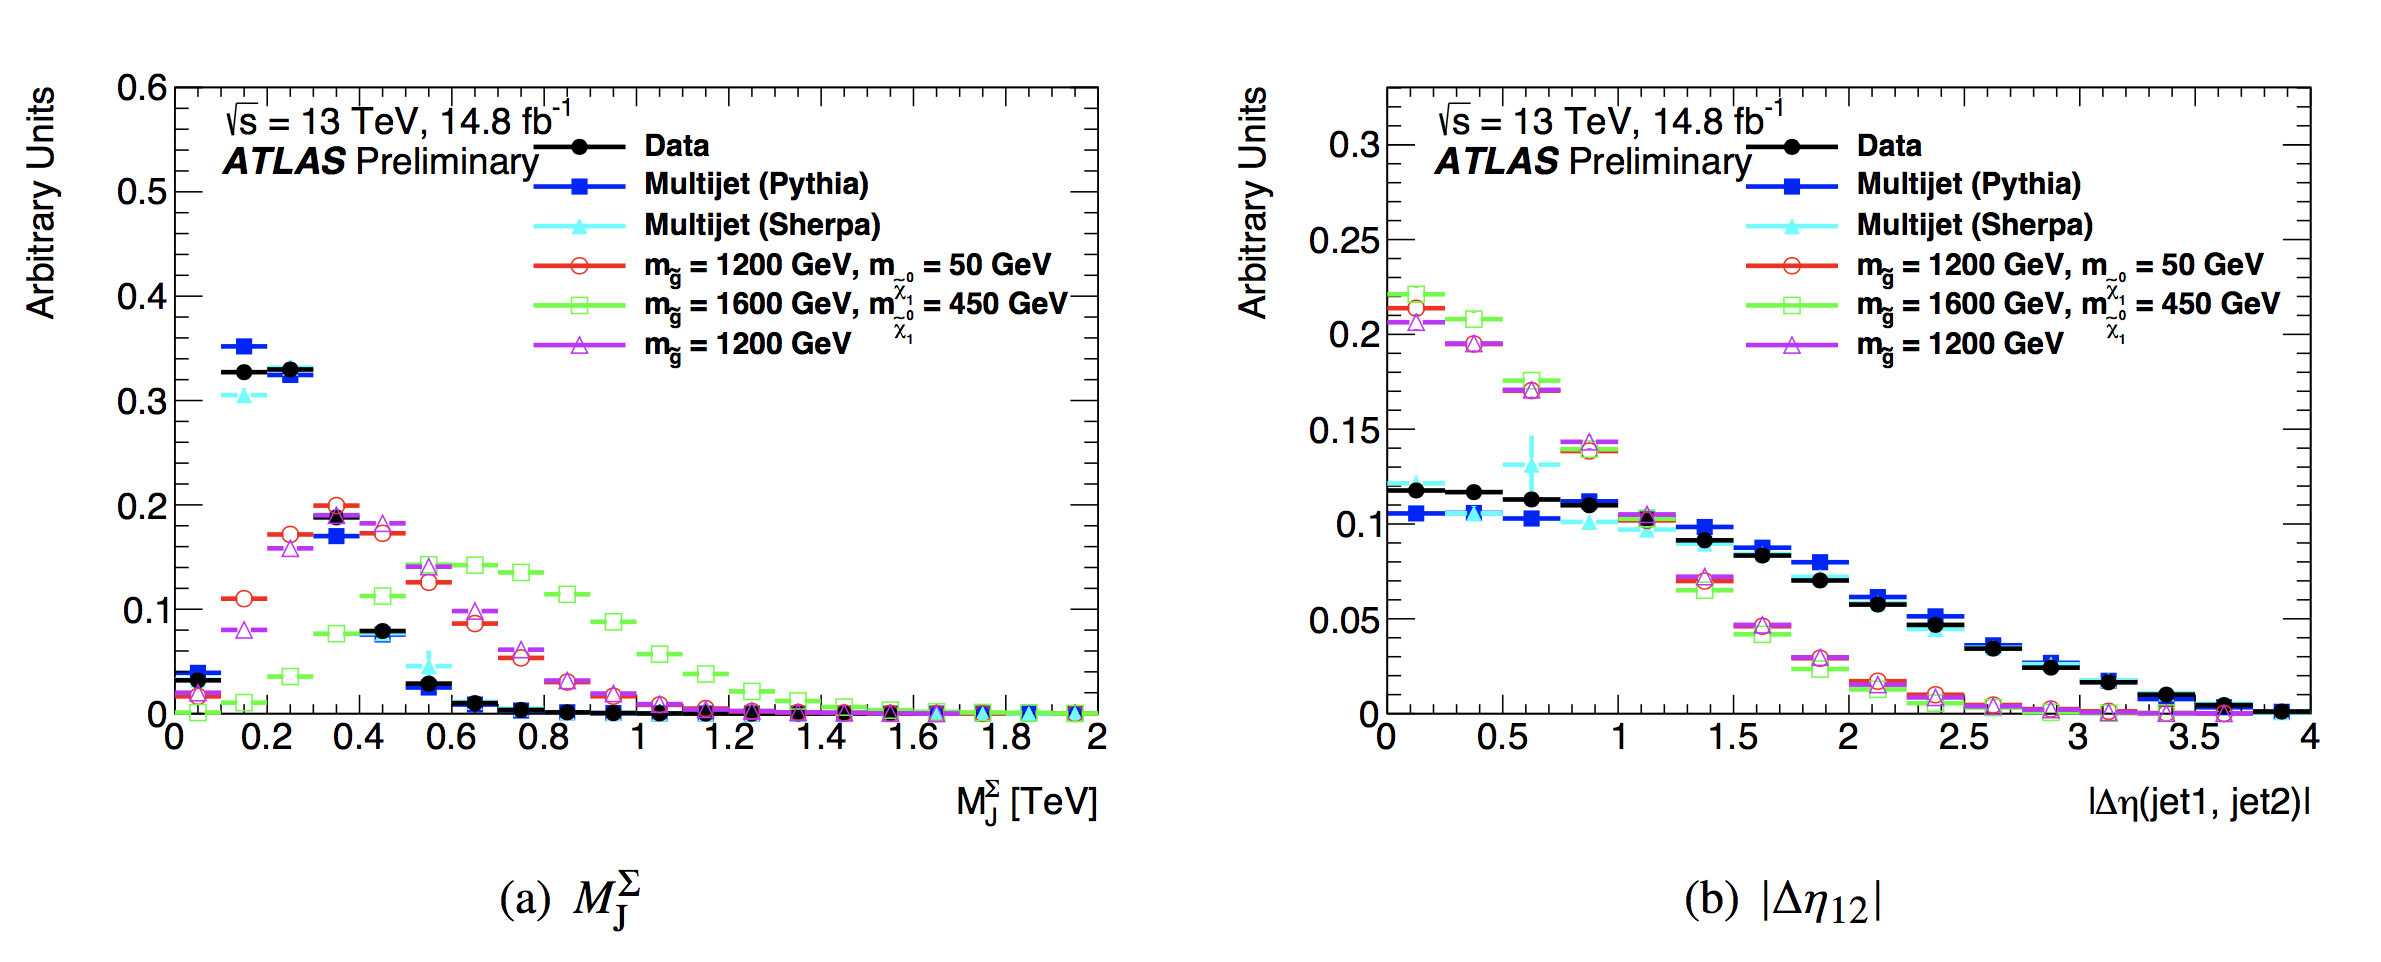
\includegraphics[width=\textwidth]{MJ_dEta_distributions_combined}
\caption{Distributions of the two main discriminating observables, (a) the scalar sum of the four leading large-R jets, $M_{J}^{\Sigma}$ and (b) the difference in pseudorapidity between the two leading jets, $|\Delta\eta_{12}|$. Selected events have $\geq 4$ large-R jets. Distributions are shown for both data and simulated signal and background samples. The red and green signal distributions are for the cascade decay mode, and the violet distribution is the direct decay mode, for the superpartner masses indicated.}
\label{fig:MJ_dEta_distributions}
\end{figure}

\section{Data-Driven Background Estimation} \label{bkg_estimation}
A data-driven jet mass template method is used to estimate the
background. The method is similar to that used in the Run-1 version of
the analysis \cite{run1-multijet}, with a
few important differences.

In the Run-1 analysis, the templates were smoothed with a kernel
density estimate before sampling the dressed masses. In this version
of the analysis, the templates remain binned. This allows for an
estimate of the statistical uncertainty from the control sample
size. By Poisson fluctuating each template bin before sampling, the
statistical uncertainty is propagated to the dressed $M_J^{\Sigma}$
distributions.

Secondly, in the Run-1 version of the analysis, two separate sets of templates
were generated: one set for the leading two jets in each event, and
one set for the third leading jet. In this analysis, the templates are
instead divided into b-matched and non-b-matched jets. The discrepancy
in template shape between b-matched and non-b-matched jets was seen to
be larger than that between the third leading jet and first two
leading jets. 

Finally, the Run-1 version of the analysis used Monte-Carlo
non-closure as one contribution to the background systematic
uncertainty. In this analysis, a data-driven method is used
instead. This is due to the fact that the sample size of available
simulated data was not large enough to make an accurate estimate of
the non-closure.

\subsection{Jet mass templates}
Jet mass templates are derived from a signal-depleted control region
consisting of events with exactly three large-R jets. For each $p_T$,
$|\eta|$, and b-match bin, the distribution of individual jet masses
in that bin is taken as the template. The templates combine to form
the binned conditional probability distribution: $p(m|p_{T}, |\eta|,
b-match)$.

Separate templates are created for b-matched and non-b-matched jets. For the b-matched templates, only events with
$|\Delta \eta_{1,2}| > 1.4$ are included in the templates. Templates
derived from b-matched jets are used to dress b-matched jets in the
kinematic sample, and templates derived from non-b-matched jets are
used to dress non-b-matched jets in the kinematic sample.

Each template is a one-dimensional histogram of $\log\left(m/p_{T}\right)$,
with $50$ bins. Jets with $\log\left(m/p_{T}\right)< -7$ are excluded
from the templates.

Example templates are shown in figure \ref{fig:template_examples} for
two representative $p_{T}$-$|\eta|$ bins. A clear difference can be
seen between the templates derived from b-matched and non-b-matched
jets. Jets that are b-matched have a higher value of $m/p_{T}$ than
non-b-matched jets, for the same  $p_{T}$-$|\eta|$ bin. This feature
can be seen in both data and simulation. Additionally,
agreement between data and simulation is observed in the general
template shapes.

\begin{figure}[h]
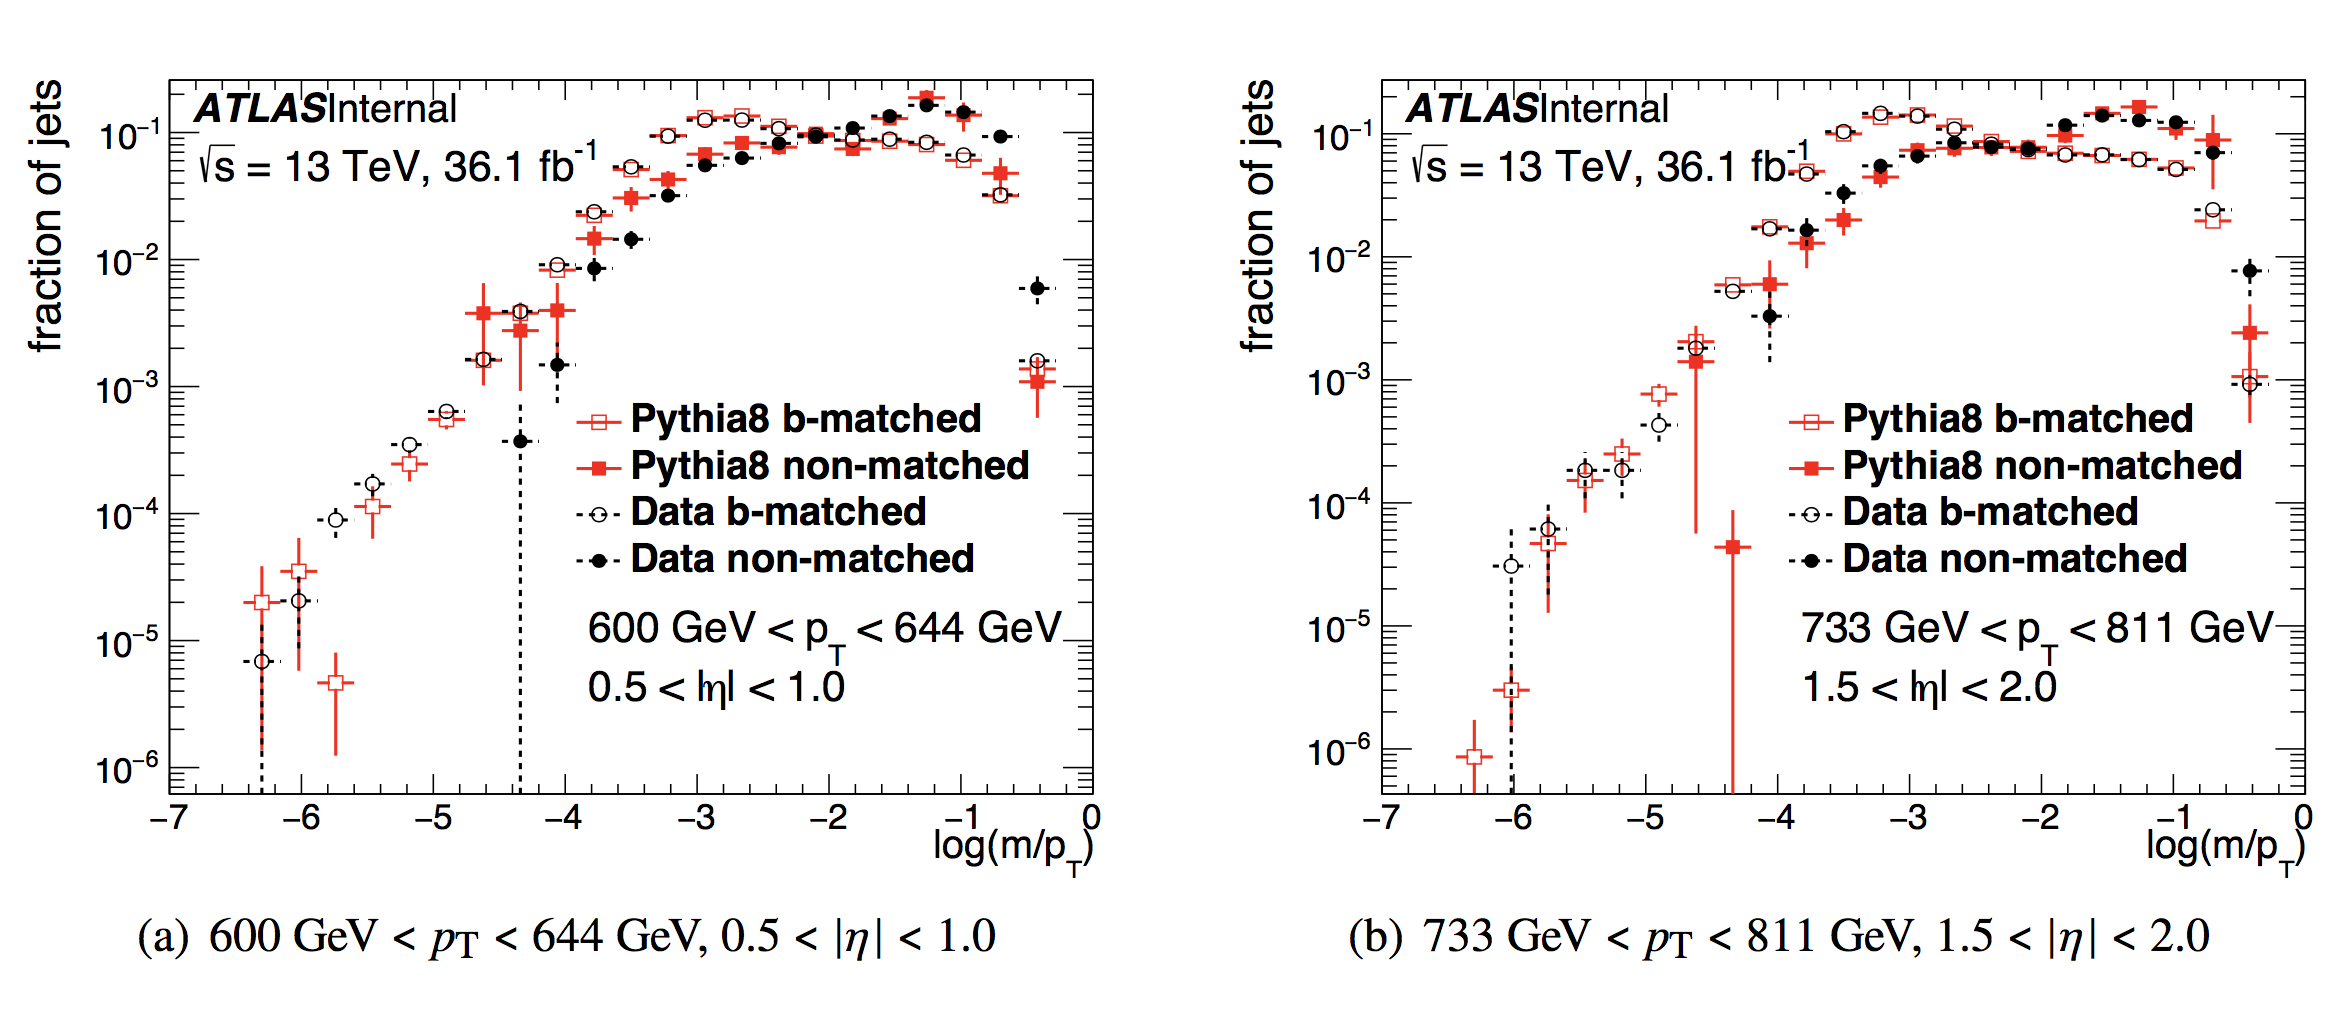
\includegraphics[width=\textwidth]{template_examples}
\caption{Two representative template distributions used in the analysis, showing a
  comparison between data in black and simulation in
  red. The solid markers show the templates derived from b-matched
  jets, while the empty markers show the templates derived from
  non-b-matched jets. In (a), template jets are required to have
  $600~GeV < p_{T} < 644~GeV$ and $0.5 <|\eta|<1.0$. In (b), templates
  jets are required to have $733~GeV < p_{T} < 811~GeV$ and $1.5<|\eta|<2.0$.}
\label{fig:template_examples}
\end{figure}

Templates are binned in $p_T$ and $|\eta|$. The $p_T$ bins are
approximately logarithmic, while the $|\eta|$ bin boundaries are at
$0.0$, $0.5$, $1.0$, and $1.5$. 

The template binning and number of jets contributing to each bin are
shown in figure \ref{fig:template_stats}.

\begin{figure}[h]
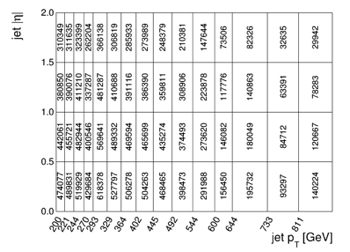
\includegraphics[width=0.5\textwidth]{template_stats_bU}
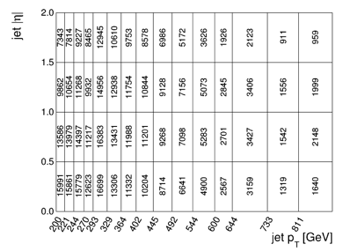
\includegraphics[width=0.5\textwidth]{template_stats_bM}
\caption{Number of jets contributing to each template bin for the
  non-b-matched (left) and b-matched (right) templates.}
\label{fig:template_stats}
\end{figure}

\subsection{Dressed mass and dressed $M_{J}^{\Sigma}$}
For each jet in the kinematic region, a dressed mass is generated by sampling from
the template corresponding to its $p_T$, $|\eta|$ and b-match bin. To
generate a dressed mass, the empirical cumulative distribution fucntion (ECDF)
is calculated for the template. A uniform random number, $y$, in the
range $[0,1)$ is then
generated. The inverse of the ECDF, $\Phi^{-1}(y)$, gives a randomized
$\log\left(m/p_T\right)$ bin. A second uniform random number, $x$, is sampled from the range
$[x_1$,$x_2)$, where $x_1,x_2$ are the edges of the selected bin. The
dressed mass is then computed as $m_{dressed} = p_{T}e^x$.

To obtain a dressed $M_{J}^{\Sigma}$ for an event, one dressed mass is
generated for each jet, and the dressed masses are summed. For
events with more than four jets, only the first four leading jets are
included in the sum.

\subsubsection{Dressed $M_{J}^{\Sigma}$ distributions}
To obtain the nominal dressed $M_{J}^{\Sigma}$ distribution,
$n_{toys}$ histograms of $M_{J}^{\Sigma}$ are created, where each
histogram is generated by dressing all events in the sample once. For
each $M_{J}^{\Sigma}$ bin, the average bin content over all histograms is taken
as the nominal value, and the standard deviation of bin contents is
taken as one contribution to the statistical uncertainty.

The $M_{J}^{\Sigma}$ histograms are binned in the following
manner. There are ten equal-width bins covering the range $0~TeV \leq M_{J}^{\Sigma} <
0.5~TeV$. The next three bins cover the ranges $0.5~TeV \leq M_{J}^{\Sigma} <
0.6~TeV$, $0.6~TeV \leq M_{J}^{\Sigma} <
0.8~TeV$, and $0.8~TeV \leq M_{J}^{\Sigma} <
1.0~TeV$. The final bin is $M_{J}^{\Sigma} \geq
1.0~TeV$

\subsubsection{Normalization}
The dressed $M_{J}^{\Sigma}$ distributions are scaled such that the
dressed yield in the range  $0.2~TeV < M_{J}^{\Sigma} <
0.4~TeV$ is equal to the kinematic yield in the same range. Separate
scale factors are derived for each of the validation and signal regions.

\subsubsection{Calculating nominal and systematically-shifted
  predictions}
To determine the nominal predicted background yield, one thousand toys
are generated, where a toy consists of a dressed $M_{J}^{\Sigma}$ value for
each event in the kinematic sample. For each toy, the number of events
with dressed $M_{J}^{\Sigma}$ greater than the signal region
$M_{J}^{\Sigma}$ cut are counted, giving a distribution of one
thousand dressed background yields. The central value of this distribution is
multiplied by the scale factor to obtain the nominal background
prediction. The standard deviation of this distribution is multiplied
by the scale factor to obtain the statistical uncertainty on the
background prediction.

Systematically-shifted background yield predictions are determined by repeating
the above procedure for the systematically-shifted dressed
$M_{J}^{\Sigma}$ values. The systematic uncertainties are taken as the
difference between the nominal and systematically-shifted background
yield predictions. Scale factors are only derived from the nominal
$M_{J}^{\Sigma}$ distributions and applied to both the nominal and
systematically-shifted predictions.

The two systematic uncertainties are symmetrized by taking the maximum
of the downward-shifted and upward-shifted uncertainties.

\subsection{Dressed Mass Response} \label{response}
Dressed mass response plots are created by plotting the average
dressed and average kinematic jet mass in each $p_T$ bin. The dressed mass
response for the control region is shown in figure
\ref{fig:response_3jCR}. Good agreement between average dressed and
kinematic masses is observed in this region, because the dressing
procedure is applied to the same jets from which the templates are
derived.

Dressed mass response plots in other regions are used to evaluate how
well the mass templates generalize to events with different jet multiplicities. In the absence of
signal events, a disagreement between the average dressed and
kinematic masses would indicate that an individual jet mass is
dependent on the number of jets in that jet's event, violating
the assumptions of the template method.

A data-driven method is used to estimate the extent to which this
assumption is violated, and the size of the effect this can have on
the background estimation uncertainty. This method is described in
\ref{bkg_uncert}

\begin{figure}[h]
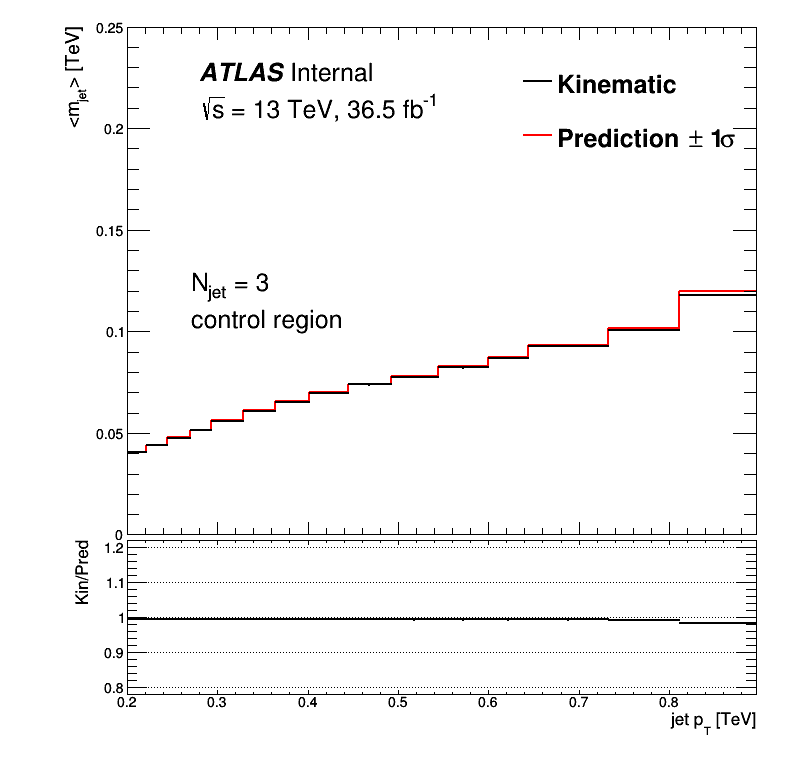
\includegraphics[width=0.6\textwidth]{plot_mass_response_3jCR}
\centering
\caption{Average dressed and kinematic jet masses for each $p_T$ bin
  in the control region}
\label{fig:response_3jCR}

\end{figure}

\section{Event Selection}
This analysis uses the entire 2015 and 2016 ATLAS datasets, comprising
$36.1~fb^{-1}~(\pm2.1\%)$. All collisions occurred as
$\sqrt{s}=13~TeV$. 

The trigger selects events with $H_{T}>1.0~TeV$, where $H_{T}$ is the
scalar sum of the $p_{T}$ of all jets in an event. The trigger
efficiency for the benchmark signal samples is found to be $100\%$.

Additional requirements are that events have a primary vertex formed
from at least two tracks with $p_{T}>400~MeV$.

Two different methods of reconstructing jets are used in the
analysis. Large-R jets are reconstructed using the anti-$k_{T}$
algorithm with radius parameter
$R=1.0$, and sub-jet radius parameter $R_{sub-jet}=0.2$. The jets are
trimmed with sub-jet $p_{T}$-fraction $f_{p_{T}}=0.05$. The details of
how jets are reconstructed, trimmed, and calibrated can be found in
chapter \ref{chapter-jets}.

Small-R jets are reconstructed with the anti-$k_{T}$ algorithm, using
radius parameter $R=0.4$. 

Large-R jets are required to have $p_{T}>200~GeV$ and
$|\eta|<2.0$. The leading large-R jet is required to have
$p_{T}>440~GeV$, a selection for which the $H_{T}$ trigger is fully
efficient.

Small-R jets are used as candidates for b-tagging. To be considered for b-tagging, a small-R jet
must have $p_{T}>50~GeV$ and $|\eta|<2.5$. The algorithm used to tag
b-jets is described in chapter \ref{chapter-jets} as well as
\cite{b-jet-perf-1, b-jet-perf-2}. The algorithm used for b-tagging in
this analysis is the fixed-efficiency $70\%$ working point.

The control, validation, and signal regions defined in section
\ref{region_defs} can be further segmented into b-tag and b-veto
regions. Events with at least one b-tagged small-R jet are considered
b-tag events, while those without are labelled as b-veto. When
b-tagging is not taken into consideration, the region is called
b-inclusive.

Additionally, large-R jets found to be within $\Delta R=1.0$ of a
b-tagged small-R jet in the same event are referred to as b-matched
jets. Those large-R jets not within $\Delta R=1.0$ of a b-tagged
small-R jet are called non-b-matched. 

The distinction in terminology between b-tagged and b-matched is important enough to
restate for clarity. When referring to the presence or absence of a b-tagged
jet \textit{within an event}, the terms b-tag, b-veto, and b-inclusive are used. When
referring to the proximity of an \textit{individual large-R jet} to a b-tagged
small-R jet, the terms b-matched and non-b-matched are used.

Templates will be divided into b-matched and non-b-matched templates,
which are used to dress b-matched and non-b-matched jets,
respectively. Validation and signal regions will be divided into
b-tag, b-veto, and b-inclusive regions.

\section{Control, Uncertainty Determination, Validation, and Signal Regions} \label{region_defs}
Events are divided into control, uncertainty determination,
validation, and signal regions.

The control region is used to derive the jet mass templates, as
described in section \ref{bkg_estimation}. The control region is
defined as those events with exactly three large-R jets. 

There are two uncertainty determination regions (UDRs), which are used to
derive the data-driven background systematic uncertainty, as detailed
in section \ref{bkg_uncert}. The high-$p_{T}$ UDR, known as UDR1,
consists of events with exactly two large-R jets, with at least one
having $p_{T}>400~GeV$. The low-$p_{T}$ UDR, known as UDR2, consists
of events with exactly four large-R jets, all of which have
$p_{T}<400~GeV$. The UDRs are independent of the control, validation,
and signal regions.

Validation region are used to check that the template method
accurately estimates the $M_J^{\Sigma}$ distribution in
high-multiplicity events that are free of signal
contamination. Requiring large $|\Delta\eta|$ reduces the signal
contribution to the high-multiplicity regions. There are four
overlapping validation regions, each requiring $|\Delta\eta| >
1.4$. The validation regions are divided into two b-tag and two
b-inclusive regions. The b-tag regions require at least one b-tagged
small-R jet, while the b-inclusive regions have no such
requirement. The b-tag and b-inclusive regions are further subdivided
into 4-jet and 5-jet regions. The 4-jet regions require \textit{at
  least} four large-R jets, and leading jet $p_T>400GeV$ so that
they are independent of UDR2. The 5-jet regions require five or more
large-R jets, and have no requirement on the leading jet $p_T$. 

The signal regions are divided the same way as the validation regions,
into two b-tag regions: one with four or more jets, and one with five
or more jets, as well as a two corresponding b-inclusive regions. The
four-jet signal regions also require lead jet $p_T>400GeV$, like the
validation region. The difference between the signal and validation
regions is a reversal of the $|\Delta\eta|$ requirement. All signal
regions require $|\Delta\eta|<1.4$. Additionally, the signal regions
include a requirement on $M_J^{\Sigma}$. The four-jet b-tag signal region
(4jSRb) and 4-jet b-inclusive signal region (4jSR) each require
$M_J^{\Sigma} > 1.0~TeV$. The five-jet b-tag signal region (5jSRb) is
divided into two overlapping regions: one with a cut of
$M_J^{\Sigma}>0.6~TeV$ and one with a cut of
$M_J^{\Sigma}>0.8~TeV$. Finally, the five-jet b-inclusive region
(5jSR) requires $M_J^{\Sigma}>0.8~TeV$.

A summary of the definitions for the control, uncertainty
determination, validation, and signal regions can be found in table \ref{tbl:region_defs}.

\begin{table}
  \caption{Summary of the requirements defining the control,
    uncertainty determination, validation, and signal
    regions. Requirements are placed on the large-R jet multiplicity
    ($N_{jet}$), the presence or absence of a b-tagged small-R jet
    ($b$-tag), the $p_T$ of the leading jet ($p_{T,1}$), the
    pseudorapidity difference between the two leading jets
    ($|\Delta\eta_{12}|$), and the scalar sum of the first four
    leading jets in the event ($M_J^{\Sigma}$).}
  \label{tbl:region_defs}
  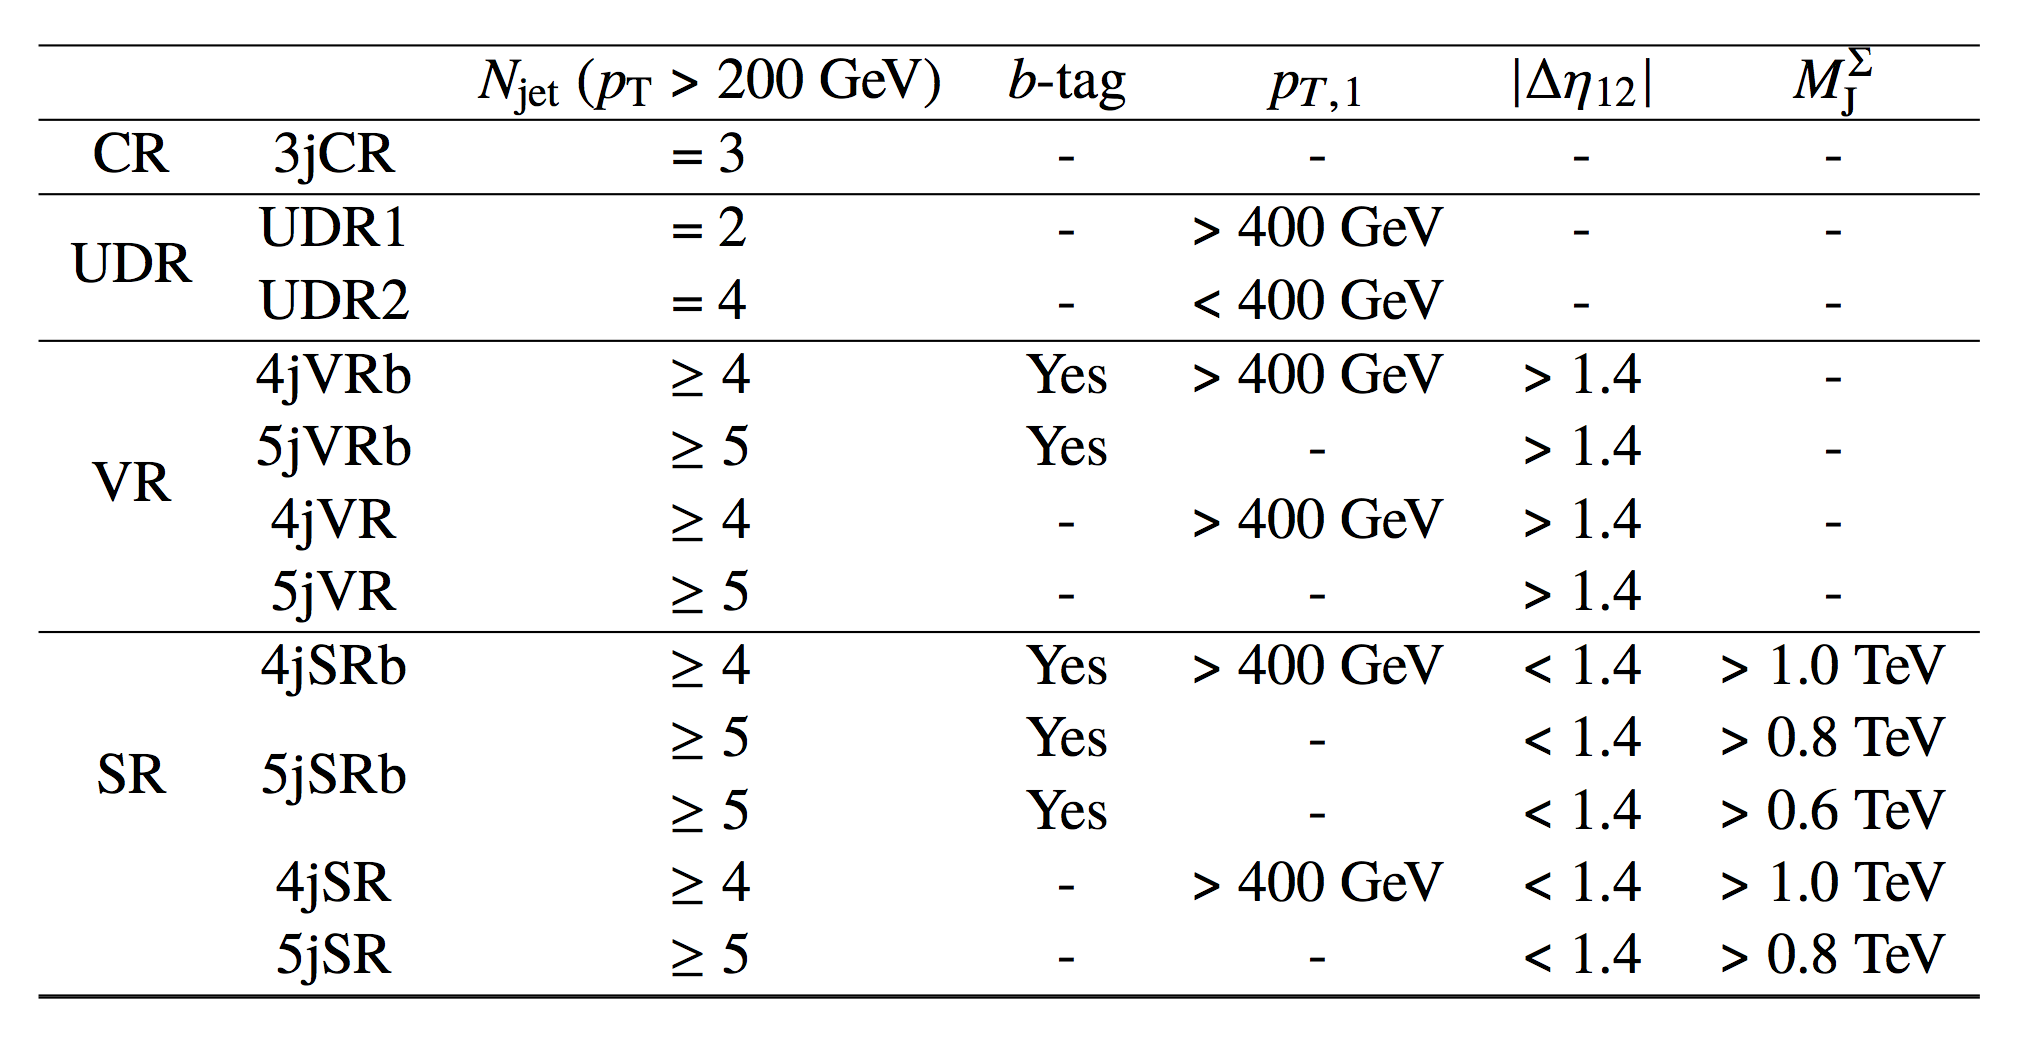
\includegraphics[width=\linewidth]{region_definition_table_2}
\end{table}

\section{Background Systematic Uncertainty} \label{bkg_uncert}
A data-driven background systematic uncertainty is derived from the
uncertainty determination regions. As can be seen in figure
\ref{fig:udr_response}, the dressing procedure tends to under-predict
jet masses in UDR1 and over-predict jet masses in UDR2. The degree of
discrepancy depends strongly on $p_T$ and the choice of UDR. Separate uncorrelated systematic uncertainties are derived
for jets with $p_T<400~GeV$ and those with $p_T<400~GeV$. Since the
discrepancy is larger in UDR1 than UDR2 for jets with $p_T<400~GeV$,
UDR1 is used to derive the uncertainty for those jets. For jets with
$p_T<400~GeV$, uncertainties are correlated across $p_T$ and $|\eta|$
bins, and likewise for jets with $p_T>400~GeV$.

\begin{figure}[h]
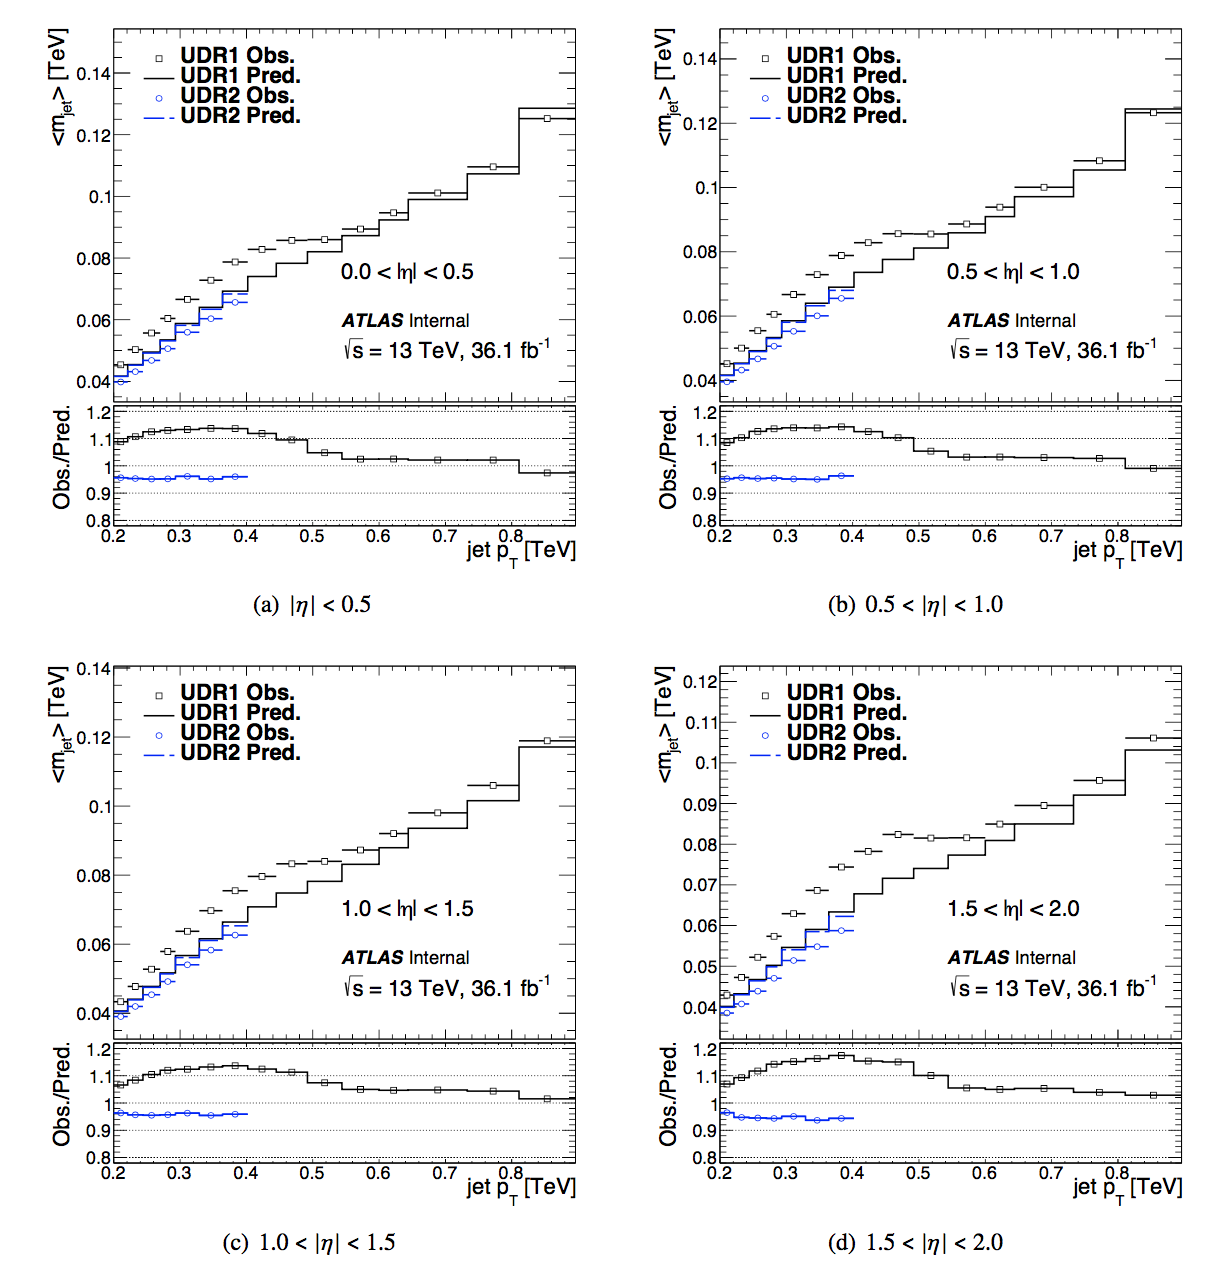
\includegraphics[width=\textwidth]{UDR_response}
\caption{Jet mass response plots showing the discrepancy between
  average dressed and kinematic jet masses in the two uncertainty
  determination regions, binned by $p_T$ and $|\eta|$. Since the
  discrepancy is always larger in UDR1, only UDR1 is used to derive
  uncertainties.}
\label{fig:udr_response}
\end{figure}

\subsubsection{Binning of systematics}
Systematic uncertainties are binned in $p_{T}$ and $|\eta|$. The lowest
$p_{T}$ bin is for jets with $p_{T} < 400~GeV$. The second bin is for
jets with $400~GeV \leq p_T
< 544~GeV$, and the highest bin is for jets with $p_T \geq 544~GeV$.

\subsubsection{Deriving uncertainty}
For jets with $p_{T} \geq 400~GeV$, uncertainties are derived only
from UDR1.

For jets with $p_{T} < 400~GeV$, uncertainties are derived from both
UDR1 and UDR2, and the maximum uncertainty is used.

For each $p_T$ bin in the UDR dressed mass response, a fractional
error is calculated as
$e_i=\left(<m_{kin}>-<m_{dressed}>\right)/<m_{dressed}>$.

For the lowest and highest $p_T$ systematic bins, the root-mean-square
of fractional errors is taken as the systematic error. For the
intermediate systematic bin, the maximum fractional error is taken

\subsubsection{Propagation of uncertainty}
Two separate, uncorrelated systematic uncertainties are derived. The first
uncertainty accounts for the discrepancy between dressed and kinematic
masses for jets with $p_T \geq 400~GeV$, and the second accounts for the
discrepancy for jets with $p_T < 400~GeV$.

To propagate the low-$p_T$ systematic, two shifted $M_{J}^{\Sigma}$
values are calculated for each dressed $M_{J}^{\Sigma}$. The first
shifted value is obtained by increasing the dressed mass of every
low-$p_T$ jet by its corresponding fractional uncertainty. This yields
$n_{toys}$ histograms of shifted $M_{J}^{\Sigma}$. The average value
of each bin content over all toys is taken to obtain the
systematically-shifted $M_{J}^{\Sigma}$ distribution. 

The second
shifted distribution is obtained by decreasing the dressed mass of every
low-$p_T$ jet by its corresponding fractional uncertainty, and
averaging over all the toys to obtain a downwards-shifted distribution
of $M_{J}^{\Sigma}$. 

The same procedure is used to propagate the high-$p_T$ systematic, but
the high-$p_T$ jets are shifted instead of the low-$p_T$ jets.



\section{Signal Contamination}
